%!TEX program = xelatex
\documentclass[11pt, a4paper]{article}
  \usepackage[a4paper,top=3cm,bottom=4cm,left=2.5cm,right=2.5cm]{geometry}
  \usepackage{subfig}
  \usepackage{graphicx}
  \graphicspath{{../images/}}
  \usepackage{hyperref}
  \usepackage{amsmath}
  \usepackage{enumitem}
  \usepackage{mathtools}
  \usepackage{xepersian}
  \settextfont[Scale=1.2]{B Nazanin}
  \setlatintextfont[Scale=1]{Times New Roman Cyr}
  \title{\textbf{شبیه‌سازی رایانه‌ای در فیزیک}\\تمرین دوم: فراکتال، لایه‌نشانی و رشد فراکتالی}
  \author{سینا معمر ۹۵۱۰۲۳۱۶}
    

\begin{document}

\maketitle
\thispagestyle{empty}


\section{\textbf{مجموعه کوخ}}
کد این بخش از تمرین در فایل
\lr{q1.py}
قابل مشاهده است. روش کار به این صورت است که ابتدا یک
\lr{object}
از کلاس
\lr{KochSnowflake}
با طول دلخواه می‌سازیم. سپس تابع
\lr{render}
را با زمان مورد نظر فراخوانی می‌کنیم. این تابع در یک حلقه به اندازه‌ی زمان داده شده، نقاط راس مرحله‌ی قبلی را به تابع
\lr{$\_\_$transform}
پاس می‌دهد و نقاط جدید را در خانه‌ی بعدی متغیر
\lr{stages$\_$points}
ذخیره می‌کند. تابع
\lr{$\_\_$transform}
به این صورت عمل می‌کند که ابتدا مختصات تمام نقاط را
$\frac{1}{3}$
کرده و بعد آن‌ها را در یک لیست جدید ذخیره می‌کند. سپس همان نقاط را به اندازه ۶۰ درجه به صورت پادساعت‌گرد می‌چرخاند و به اندازه 
$\frac{1}{3}$
طول اولیه به سمت راست منتقل می‌کند. این نقاط جدید را هم در ادامه‌‌ی نقاط قبلی در لیست ذخیره می‌کند. سپس نقاط اسکیل شده‌ی اولیه را این‌بار ۶۰ درجه به صورت ساعت‌گرد می‌چرخاند و به اندازه‌
$\frac{2}{3}$
طول اولیه به راست منتقل کرده و سپس در لیست ذخیره می‌کند. در نهایت نیز نقاط اولیه را به اندازه‌ی 
$\frac{2}{3}$
طول به راست منتقل و آن‌ها را نیز به لیست نهایی اضافه می‌کند. لیست به دست‌ آمده مختصات رئوس مرحله‌ی جدید مجموعه‌ی کوخ است و در جواب تابع برگردانده می‌شود. لازم به ذکر است که تمامی مختصات به صورت اعداد مختلط ذخیره شده‌اند و عمل انتقال از طریق جمع و عمل دوران نیز از طریق ضرب اعداد مختلط انجام شده است.
نتیجه به دست آمده تا مرحله‌ی ۵ ام را در شکل
\ref{fig:q1_koch}
می‌توان مشاهده نمود.

\begin{figure}
  \begin{tabular}{|c|c|}
    \hline
    \subfloat[مرحله‌ ۰]{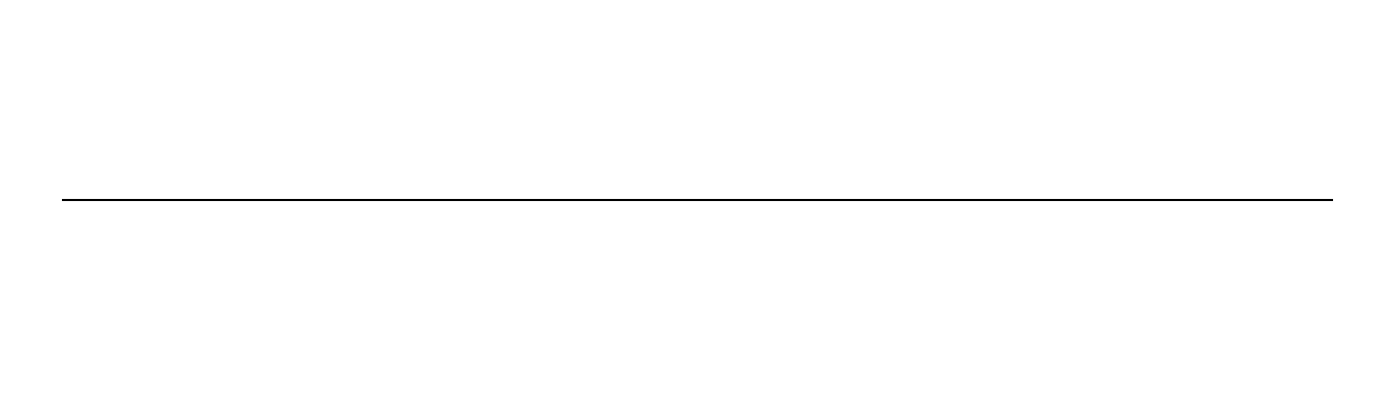
\includegraphics[width=.45\textwidth]{q1-stage-0.png}} &
    \subfloat[مرحله ۱]{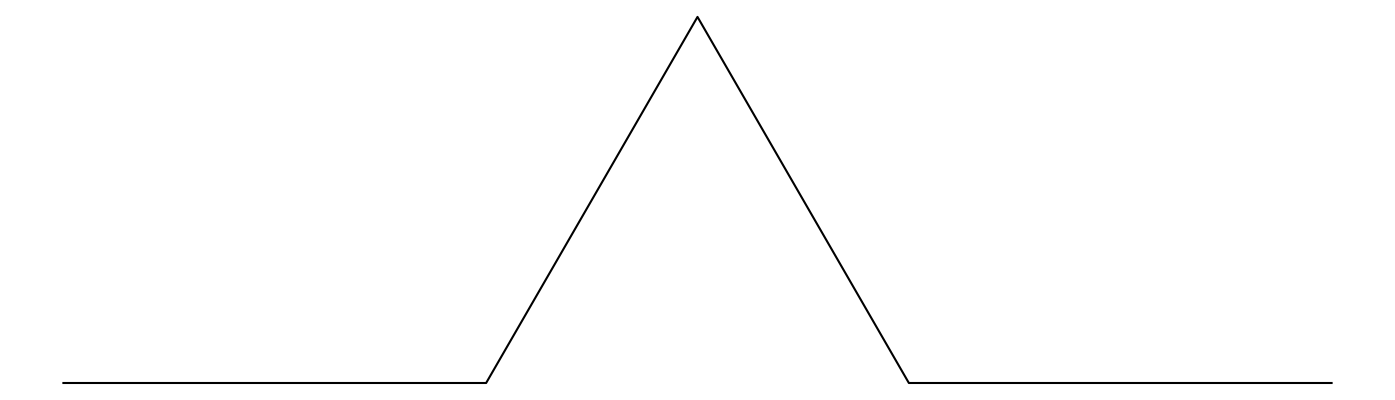
\includegraphics[width=.45\textwidth]{q1-stage-1.png}} \\
    \hline
    \subfloat[مرحله‌ ۲]{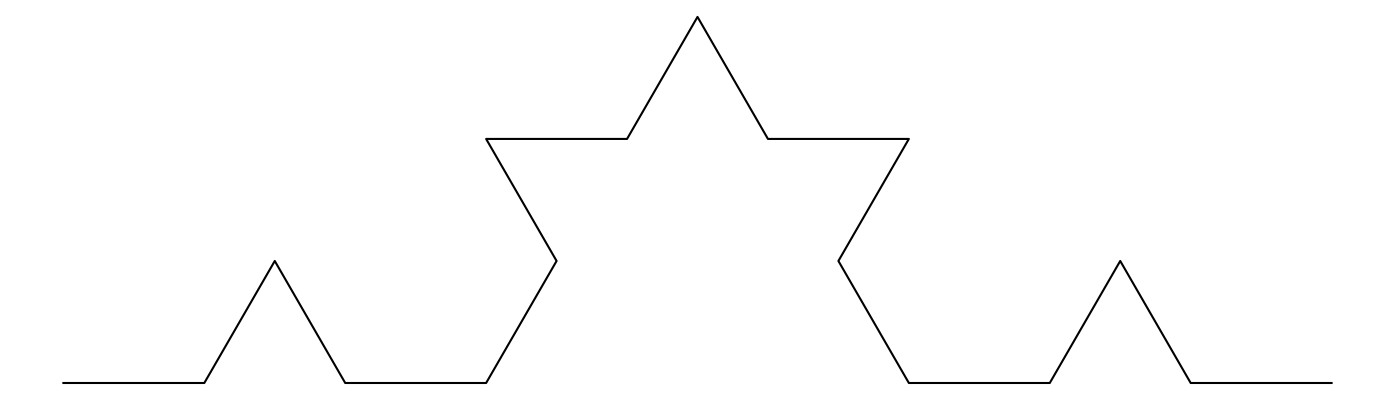
\includegraphics[width=.45\textwidth]{q1-stage-2.png}} &
    \subfloat[مرحله ۳]{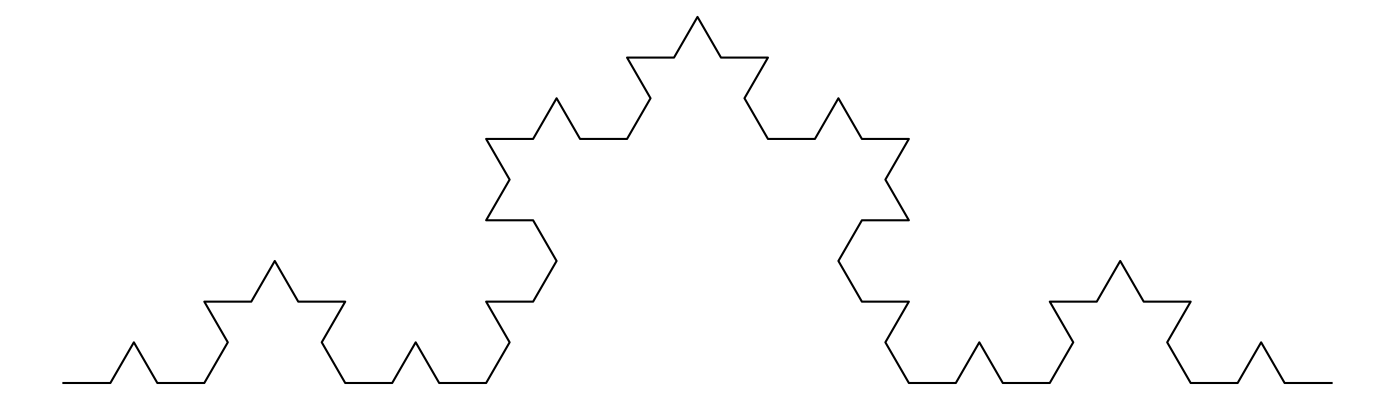
\includegraphics[width=.45\textwidth]{q1-stage-3.png}} \\
    \hline
    \subfloat[مرحله‌ ۴]{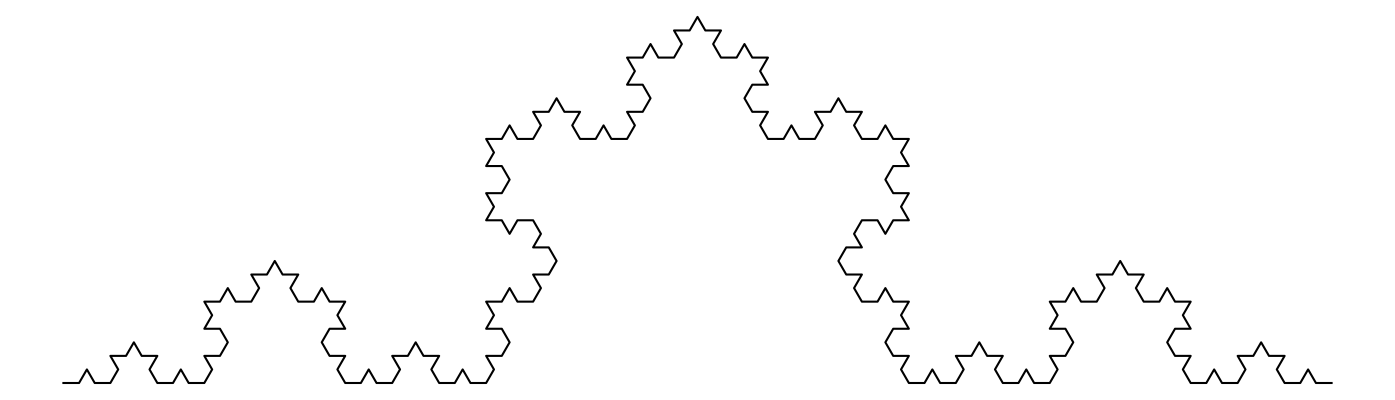
\includegraphics[width=.45\textwidth]{q1-stage-4.png}} &
    \subfloat[مرحله ۵]{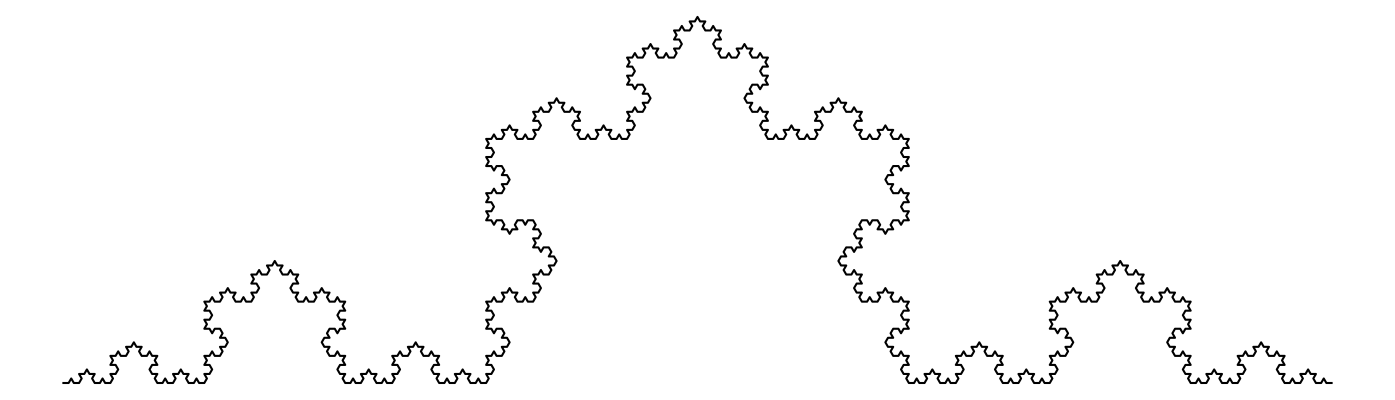
\includegraphics[width=.45\textwidth]{q1-stage-5.png}} \\
    \hline
  \end{tabular}
  \caption{مجموعه کوخ تا مرحله ۵ ام}
  \label{fig:q1_koch}
\end{figure}


\section{\textbf{مثلث سرپینسکی}}
کد این بخش از تمرین در فایل
\lr{q2.py}
قابل مشاهده است. روش کار به این صورت است که ابتدا یک
\lr{object}
از کلاس
\lr{SierpinskiTriangle}
با طول دلخواه می‌سازیم. سپس تابع
\lr{render}
را با زمان مورد نظر فراخوانی می‌کنیم. این تابع در یک حلقه به اندازه‌ی زمان داده شده، نقاط راس مرحله‌ی قبلی را به تابع
\lr{$\_\_$transform}
پاس می‌دهد و نقاط جدید را در خانه‌ی بعدی متغیر
\lr{stages$\_$points}
ذخیره می‌کند. تابع
\lr{$\_\_$transform}
به این صورت عمل می‌کند که ابتدا مختصات تمام نقاط را
$\frac{1}{2}$
کرده و بعد آن‌ها را در یک لیست جدید ذخیره می‌کند. سپس همان نقاط را به اندازه 
$\frac{1}{2}$
طول اولیه به سمت راست منتقل می‌کند. این نقاط جدید را هم در ادامه‌‌ی نقاط قبلی در لیست ذخیره می‌کند. سپس نقاط اسکیل شده‌ی اولیه را این‌بار به اندازه‌
$\frac{1}{4}$
طول اولیه به راست و به اندازه‌ی 
$\frac{\sqrt{3}}{4}$
طول به بالا منتقل کرده و آن‌ها را نیز به لیست نهایی اضافه می‌کند. لیست به دست‌ آمده مختصات رئوس مرحله‌ی جدید مثلث سرپینسکی است و در جواب تابع برگردانده می‌شود. لازم به ذکر است که تمامی مختصات به صورت اعداد مختلط ذخیره شده‌اند و عمل انتقال از طریق جمع و عمل دوران نیز از طریق ضرب اعداد مختلط انجام شده است.
نتیجه به دست آمده تا مرحله‌ی ۵ ام را در شکل
\ref{fig:q2_sierpinski}
می‌توان مشاهده نمود.

\begin{figure}
  \begin{tabular}{|c|c|c|}
    \hline
    \subfloat[مرحله‌ ۰]{
\includegraphics[width=.3\textwidth]{q2-stage-0.png}} &
    \subfloat[مرحله ۱]{
\includegraphics[width=.3\textwidth]{q2-stage-1.png}} &
    \subfloat[مرحله‌ ۲]{
\includegraphics[width=.3\textwidth]{q2-stage-2.png}} \\
    \hline
    \subfloat[مرحله ۳]{
\includegraphics[width=.3\textwidth]{q2-stage-3.png}} &
    \subfloat[مرحله‌ ۴]{
\includegraphics[width=.3\textwidth]{q2-stage-4.png}} &
    \subfloat[مرحله ۵]{
\includegraphics[width=.3\textwidth]{q2-stage-5.png}} \\
    \hline
  \end{tabular}
  \caption{مثلث سرپینسکی تا مرحله ۵ ام}
  \label{fig:q2_sierpinski}
\end{figure}


\section{\textbf{مثلث سرپینسکی (الگوریتم تصادفی)}}
کد این بخش از تمرین در فایل
\lr{q3.py}
قابل مشاهده است. روش کار به این صورت است که ابتدا یک
\lr{object}
از کلاس
\lr{RandomSierpinskiTriangle}
با تعداد نقاط دلخواه می‌سازیم. سپس تابع
\lr{render}
را با زمان مورد نظر فراخوانی می‌کنیم. این تابع در ابتدا با استفاده از تابع
\lr{$\_\_$random$\_$points}
به اندازه‌ی تعداد داده شده، نقاط با مختصات تصادفی در مثلث دلخواه تولید می‌کند.
برای این کار نقاط را از یک مستطیل به عرض
$\frac{1}{2}$
و ارتفاع
$\frac{\sqrt{3}}{2}$
ضلع مثلث انتخاب می‌کند و نقاط بالاتر از قطر را معادل با نقاط نیمه دوم در نظر می‌گیرد.
پس از تولید این نقاط، تابع
\lr{render}
در یک حلقه به اندازه‌ی زمان داده شده، نقاط راس مرحله‌ی قبلی را به تابع
\lr{$\_\_$random$\_$transform}
پاس می‌دهد و نقاط جدید را در خانه‌ی بعدی متغیر
\lr{stages$\_$points}
ذخیره می‌کند. تابع
\lr{$\_\_$random$\_$transform}
به این صورت عمل می‌کند که ابتدا از بین ۳ نوع تبدیل خود‌متشابه‌ای که برای مثلث سرپینسکی وجود دارد،
به طور تصادفی و به اندازه‌ی تعداد نقاط داده شده، تبدیل انتخاب می‌کند و آن‌ها را بر روی نقاط اولیه اثر می‌دهد.
این تبدیل‌ها همان تبدیل‌هایی هستند که در سوال قبلی توضیح داده شده‌اند.
لازم به ذکر است که تمامی مختصات به صورت اعداد مختلط ذخیره شده‌اند
و عمل انتقال از طریق جمع و عمل دوران نیز از طریق ضرب اعداد مختلط انجام شده است.
نتیجه به دست آمده برای مرحله‌ی ۹ ام و با
$1\,000\,000$
نقطه را در شکل
\ref{fig:q3_sierpinski_random}
می‌توان مشاهده نمود.

\begin{figure}[h]
  \centering
  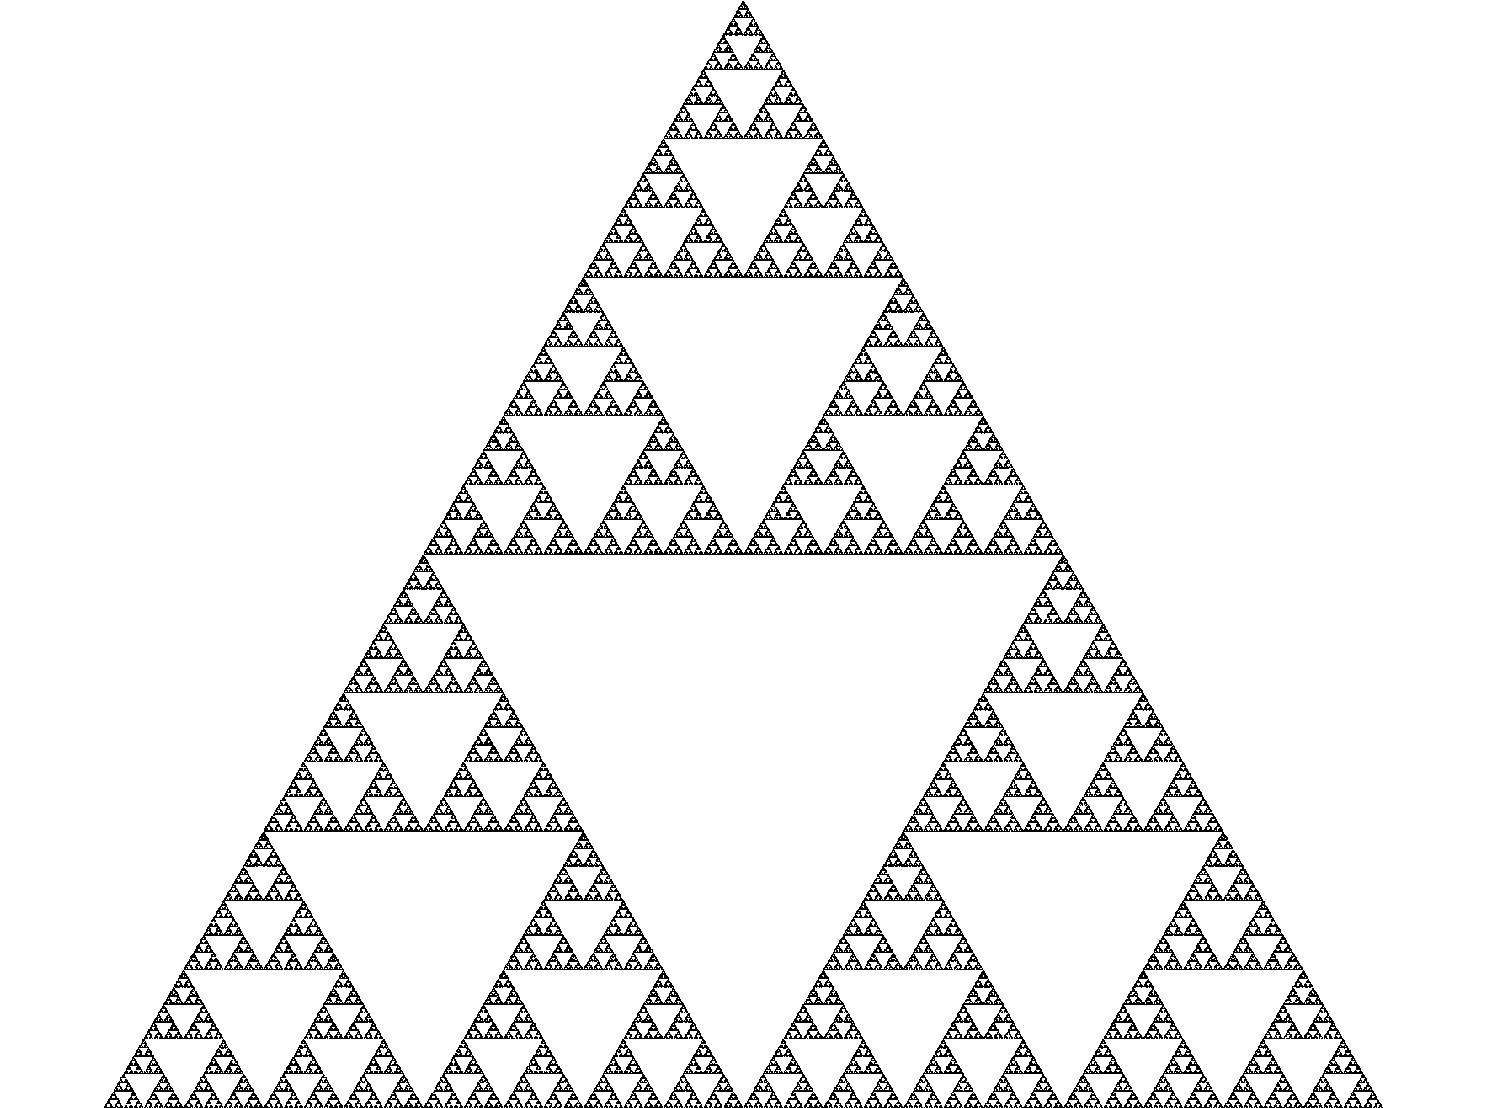
\includegraphics[width=.5\textwidth]{q3_1000000_9.png}
  \caption{مثلث سرپینسکی با الگوریتم تصادفی در مرحله‌ی ۹ با $1\,000\,000$ نقطه}
  \label{fig:q3_sierpinski_random}
\end{figure}


\section{\textbf{ول‌نشست}}
کد این بخش از تمرین در فایل
\lr{q4.py}
قابل مشاهده است. روش کار به این صورت است که ابتدا یک
\lr{object}
از کلاس
\lr{RandomBallisticDeposition}
با طول دلخواه می‌سازیم. سپس تابع
\lr{render}
را با زمان مورد نظر فراخوانی می‌کنیم. روش کار این تابع به این صورت است که روی بازه‌های زمانی داده شده
پیمایش می‌کند و در هر بازه، به اندازه‌ی طول آن، اعداد تصادفی از مجموعه‌ی اندیس‌ها تولید می‌کند. 
سپس تعداد تکرار هر یک از اندیس‌ها را می‌شمارد و به ارتفاع آن خانه اضافه می‌کند.
در نهایت داده‌های به دست آمده را در یک فایل به فرمت
\lr{.npy}
ذخیره می‌کند.
برای رسم تصویر داده‌ها باید تابع
\lr{show}
را صدا بزنیم.
تصویر به دست آمده برای طول
$200$
و زمان
$20\,000$
را در شکل
\ref{fig:q4_201_20000}
می‌توان مشاهده نمود.
\\
برای ایجاد یک آنسامبل آماری، می توانیم تابع
\lr{make$\_$ensemble}
را با بازه‌ی زمانی و تعداد دلخواه فراخوانی کنیم. 
این تابع به تعداد داده شده، تابع
\lr{render}
را صدا می‌زند و در نهایت میانگین ارتفاع و 
$\omega$
را برای این آنسامبل محاسبه کرده و در یک فایل ذخیره می‌کند.
برای انجام تحلیل بر روی این داده‌های به دست آمده و محاسبه شیب رشد، تابع
\lr{analyse}
را صدا می‌زنیم.
منحنی تغییرات ناهمواری و میانگین ارتفاع بر حسب زمان را برای ول‌نشستی به طول
$200$
و با
$200$
تکرار را در شکل‌های
\ref{fig:q4_200_200_omega}
و
\ref{fig:q4_200_200_avg}
می‌توان مشاهده نمود.
\\
شیب خط فیت شده به این دو منحنی را در جدول
\ref{tab:q4_slope}
همراه با خطا‌ی محاسبه‌شان آورده شده است.

\begin{figure}[h]
  \centering
  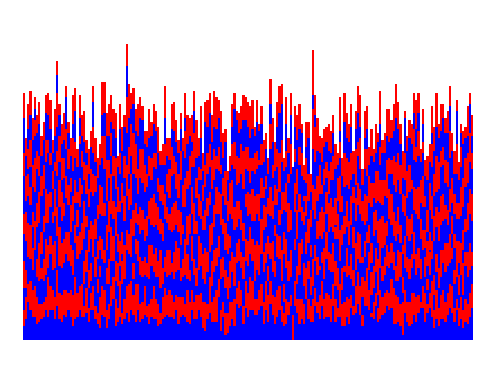
\includegraphics[width=.5\textwidth]{q4_201_20000.png}
  \caption{ول‌نشست به طول $200$ و زمان $20\,000$}
  \label{fig:q4_201_20000}
\end{figure}

\begin{figure}[h]
	\centering
  \begin{minipage}[b]{0.48\textwidth}
    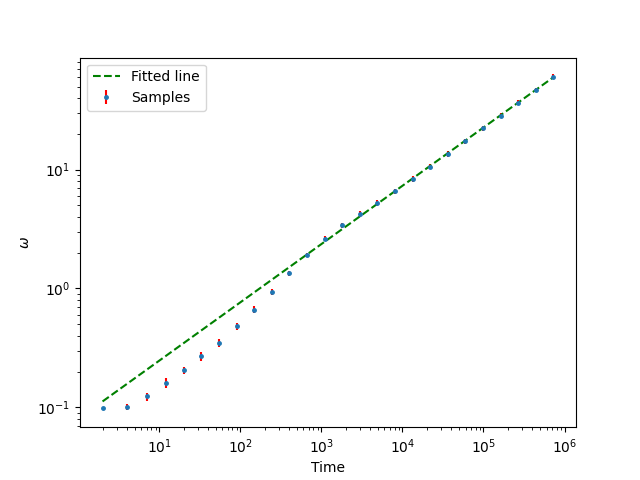
\includegraphics[width=\textwidth]{q4_200_200_1_14_.5_omega.png}
    \caption{منحنی تغییرات ناهمواری بر حسب زمان برای ول‌نشستی به طول $200$ و با $200$ بار تکرار}
    \label{fig:q4_200_200_omega}
  \end{minipage}
  \hfill
  \begin{minipage}[b]{0.48\textwidth}
    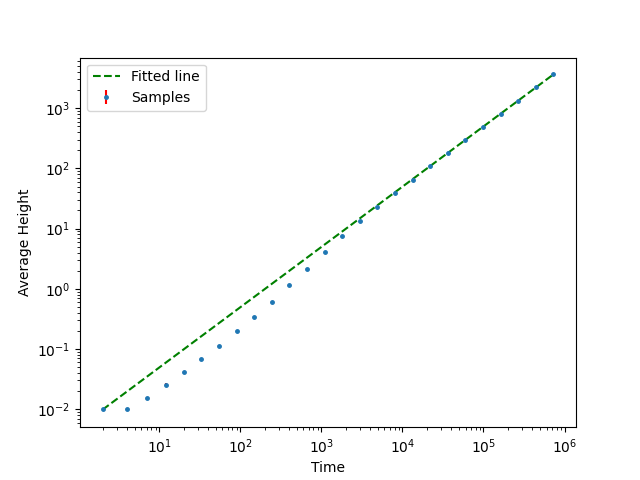
\includegraphics[width=\textwidth]{q4_200_200_1_14_.5_avg.png}
    \caption{منحنی تغییرات میانگین ارتفاع بر حسب زمان برای ول‌نشستی به طول $200$ و با $200$ بار تکرار}
    \label{fig:q4_200_200_avg}
  \end{minipage}
\end{figure}

\begin{table}[h]
	\centering
	\begin{tabular}{|c|c|}
		\hline
    $1.001406 \pm 10^{-6}$ & \text{میانگین ارتفاع} \\
     \hline
    $\beta = 0.4904 \pm 10^{-4}$ & \text{ناهمواری } ($\omega$) \\
     \hline
	\end{tabular}
	\caption{شیب خطوط فیت شده به منحنی تغییرات میانگین ارتفاع و ناهمواری ول‌نشستی به طول ۲۰۰}
	\label{tab:q4_slope}
\end{table}


\section{\textbf{پایین‌نشست}}
کد این بخش از تمرین در فایل
\lr{q5.py}
قابل مشاهده است. روش کار به این صورت است که ابتدا یک
\lr{object}
از کلاس
\lr{RandomBallisticWithRelaxation}
با طول دلخواه می‌سازیم. سپس تابع
\lr{render}
را با زمان مورد نظر فراخوانی می‌کنیم. روش کار این تابع به این صورت است که روی بازه‌های زمانی داده شده
پیمایش می‌کند و در هر بازه، به اندازه‌ی طول آن، اعداد تصادفی از مجموعه اندیس‌ها تولید می‌کند. 
سپس روی این اندیس‌های تصادفی پیمایش می‌کند و کمترین ارتفاع را در همسایگی آن پیدا کرده و ارتفاع آن خانه را یکی افزایش می‌دهد.
در نهایت داده‌های به دست آمده را در یک فایل به فرمت
\lr{.npy}
ذخیره می‌کند.
برای رسم تصویر داده‌ها باید تابع
\lr{show}
را صدا بزنیم.
تصویر به دست آمده برای طول
$200$
و زمان
$20\,000$
را در شکل
\ref{fig:q5_201_20000}
می‌توان مشاهده نمود.
\\
برای ایجاد یک آنسامبل آماری، می توانیم تابع
\lr{make$\_$ensemble}
را با بازه‌ی زمانی و تعداد دلخواه فراخوانی کنیم. 
این تابع به تعداد داده شده، تابع
\lr{render}
را صدا می‌زند و در نهایت میانگین ارتفاع و 
$\omega$
را برای این آنسامبل محاسبه کرده و در یک فایل ذخیره می‌کند.
برای انجام تحلیل بر روی این داده‌های به دست آمده و محاسبه شیب رشد، تابع
\lr{analyse}
را صدا می‌زنیم.
منحنی تغییرات ناهمواری و میانگین ارتفاع بر حسب زمان را برای ول‌نشستی به طول
$200$
و با
$50$
تکرار را در شکل‌های
\ref{fig:q5_200_50_omega}
و
\ref{fig:q5_200_50_avg}
می‌توان مشاهده نمود. همان‌طور که دیده می‌شود، برای مشاهده‌ی رفتار اشباع، به بیش از
$100\,000$
ذره نیاز است.
\\
شیب خط فیت شده به این دو منحنی و مقدار اشباع برای طول‌های مختلف را در جدول
\ref{tab:q5_slope}
همراه با خطا‌ی محاسبه‌شان آورده شده است.
با توجه مقادیر اشباع به دست آمده، منحنی تغییرات اشباع بر حسب طول را در شکل
\ref{fig:q5_z}
رسم می‌کنیم. شیب خط فیت شده به آن برابر است با:

\begin{equation}
  \alpha = 0.4986 \pm 10^{-4}
  \label{eqn:q5_z}
\end{equation}

\begin{equation}
  \alpha = z \beta
  \xRightarrow{\eqref{eqn:q5_z}}
  z = 2.046 \pm 10^{-3}
\end{equation}

\begin{figure}[h]
  \centering
  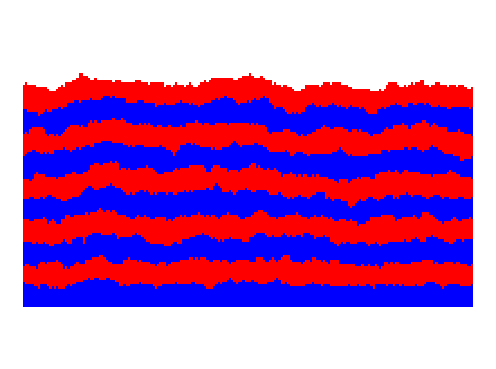
\includegraphics[width=.5\textwidth]{q5_201_20000.png}
  \caption{پایین‌نشست به طول $200$ و زمان $20\,000$}
  \label{fig:q5_201_20000}
\end{figure}

\begin{figure}[h]
	\centering
  \begin{minipage}[b]{0.48\textwidth}
    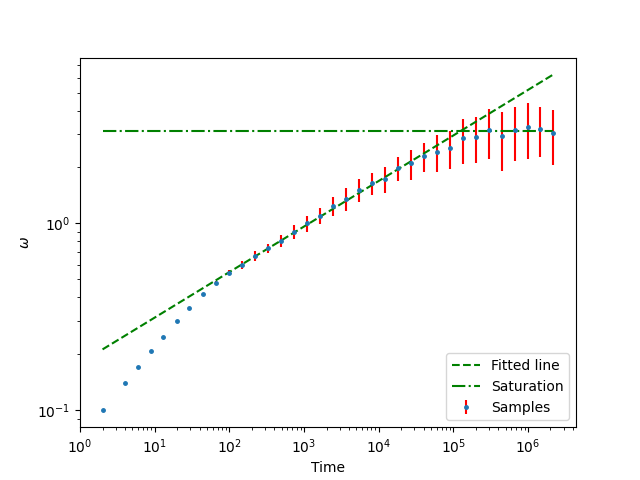
\includegraphics[width=\textwidth]{q5_200_50_1_15_.4_omega.png}
    \caption{منحنی تغییرات ناهمواری بر حسب زمان برای پایین‌نشستی به طول $200$ و با $50$ بار تکرار}
    \label{fig:q5_200_50_omega}
  \end{minipage}
  \hfill
  \begin{minipage}[b]{0.48\textwidth}
    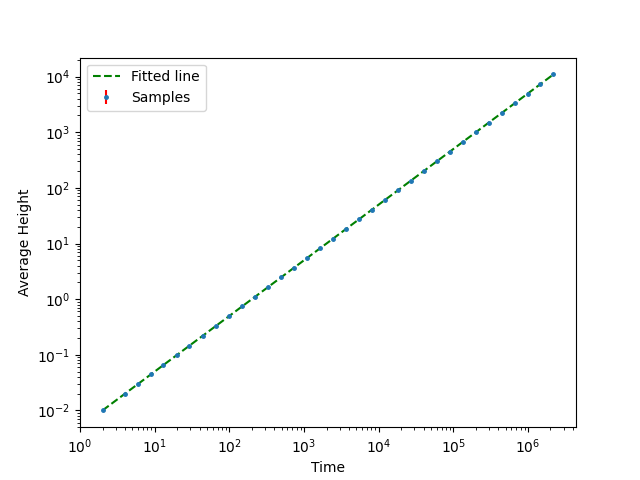
\includegraphics[width=\textwidth]{q5_200_50_1_15_.4_avg.png}
    \caption{منحنی تغییرات میانگین ارتفاع بر حسب زمان برای پایین‌نشستی به طول $200$ و با $50$ بار تکرار}
    \label{fig:q5_200_50_avg}
  \end{minipage}
\end{figure}

\begin{table}[h]
	\centering
	\begin{tabular}{|c|c|c|c|}
    \hline
    \text{طول } ($l$) & \text{میانگین ارتفاع} & \text{ناهمواری } ($\omega$) & \text{اشباع } ($\omega_s$) \\
    \hline
    $200$ & $1.0 \pm 10^{-32}$ & $\beta = 0.24366 \pm 10^{-5}$ & $3.124 \pm 10^{-3}$ \\
    \hline
    $150$ & $1.0 \pm 10^{-32}$ & $\beta = 0.2428 \pm 10^{-4}$ & $2.655 \pm 10^{-3}$ \\
    \hline
    $100$ & $1.0 \pm 10^{-32}$ & $\beta = 0.2363 \pm 10^{-4}$ & $2.168 \pm 10^{-3}$ \\
    \hline
    $50$ & $1.0 \pm 10^{-31}$ & $\beta = 0.2320 \pm 10^{-4}$ & $1.5575 \pm 10^{-4}$ \\
    \hline
	\end{tabular}
	\caption{شیب خطوط فیت شده به منحنی تغییرات میانگین ارتفاع و ناهمواری و مقدار اشباع برای طول‌های مختلف پایین‌نشست}
	\label{tab:q5_slope}
\end{table}

\begin{figure}[h]
  \centering
  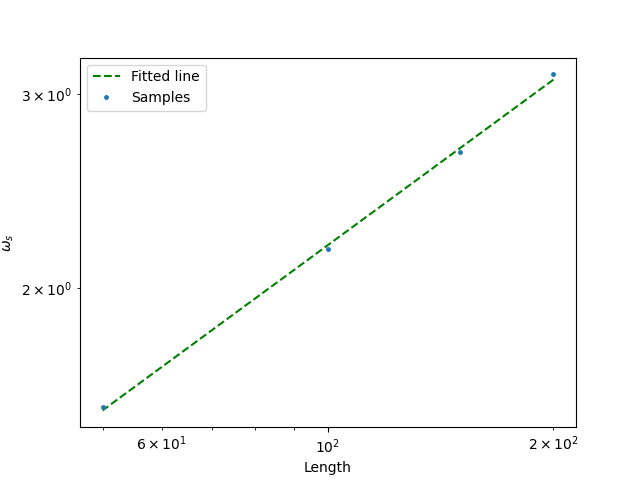
\includegraphics[width=.5\textwidth]{q5_z.png}
  \caption{منحنی تغییرات اشباع بر حسب طول پایین‌نشست}
  \label{fig:q5_z}
\end{figure}


\section{\textbf{کنارنشست}}
کد این بخش از تمرین در فایل
\lr{q6.py}
قابل مشاهده است. روش کار به این صورت است که ابتدا یک
\lr{object}
از کلاس
\lr{NearestNeighborBallisticDeposition}
با طول دلخواه می‌سازیم. سپس تابع
\lr{render}
را با زمان مورد نظر فراخوانی می‌کنیم. روش کار این تابع به این صورت است که روی بازه‌های زمانی داده شده
پیمایش می‌کند و در هر بازه، به اندازه‌ی طول آن، اعداد تصادفی از مجموعه اندیس‌ها تولید می‌کند. 
سپس روی این اندیس‌های تصادفی پیمایش می‌کند و بیش‌ترین ارتفاع را در همسایگی آن پیدا کرده و ارتفاع آن خانه را برابر با آن قرار می‌دهد.
در نهایت داده‌های به دست آمده را در یک فایل به فرمت
\lr{.npy}
ذخیره می‌کند.
برای رسم تصویر داده‌ها باید تابع
\lr{show}
را صدا بزنیم.
تصویر به دست آمده برای طول
$200$
و زمان
$20\,000$
را در شکل
\ref{fig:q6_200_20000}
می‌توان مشاهده نمود.
\\
برای ایجاد یک آنسامبل آماری، می توانیم تابع
\lr{make$\_$ensemble}
را با بازه‌ی زمانی و تعداد دلخواه فراخوانی کنیم. 
این تابع به تعداد داده شده، تابع
\lr{render}
را صدا می‌زند و در نهایت میانگین ارتفاع و 
$\omega$
را برای این آنسامبل محاسبه کرده و در یک فایل ذخیره می‌کند.
برای انجام تحلیل بر روی این داده‌های به دست آمده و محاسبه شیب رشد، تابع
\lr{analyse}
را صدا می‌زنیم.
منحنی تغییرات ناهمواری و میانگین ارتفاع بر حسب زمان را برای کنارنشستی به طول
$200$
و با
$50$
تکرار را در شکل‌های
\ref{fig:q6_200_50_omega}
و
\ref{fig:q6_200_50_avg}
می‌توان مشاهده نمود.
\\
شیب خط فیت شده به این دو منحنی و مقدار اشباع برای طول‌های مختلف را در جدول
\ref{tab:q6_slope}
همراه با خطا‌ی محاسبه‌شان آورده شده است.
با توجه به مقادیر اشباع به دست آمده، منحنی تغییرات اشباع بر حسب طول را در شکل
\ref{fig:q6_z}
رسم می‌کنیم. شیب خط فیت شده به آن برابر است با:

\begin{equation}
  \alpha = 0.460 \pm 10^{-3}
  \label{eqn:q6_z}
\end{equation}

\begin{equation}
  \alpha = z \beta
  \xRightarrow{\eqref{eqn:q6_z}}
  z = 2.10 \pm 10^{-2}
\end{equation}

\begin{figure}[h]
  \centering
  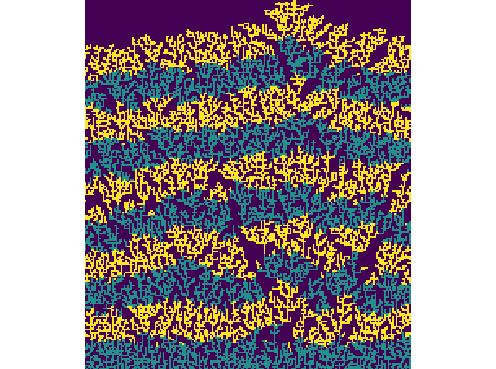
\includegraphics[width=.5\textwidth]{q6_200_20000.png}
  \caption{کنارنشست به طول $200$ و زمان $20\,000$}
  \label{fig:q6_200_20000}
\end{figure}

\begin{figure}[h]
	\centering
  \begin{minipage}[b]{0.48\textwidth}
    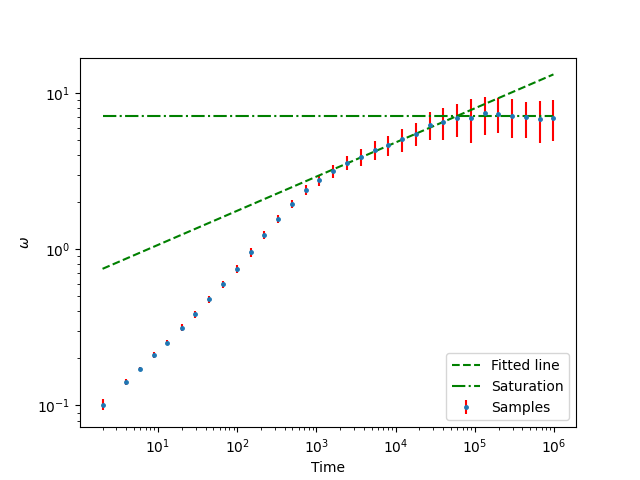
\includegraphics[width=\textwidth]{q6_200_50_1_14_.4_omega.png}
    \caption{منحنی تغییرات ناهمواری بر حسب زمان برای کنارنشستی به طول $200$ و با $50$ بار تکرار}
    \label{fig:q6_200_50_omega}
  \end{minipage}
  \hfill
  \begin{minipage}[b]{0.48\textwidth}
    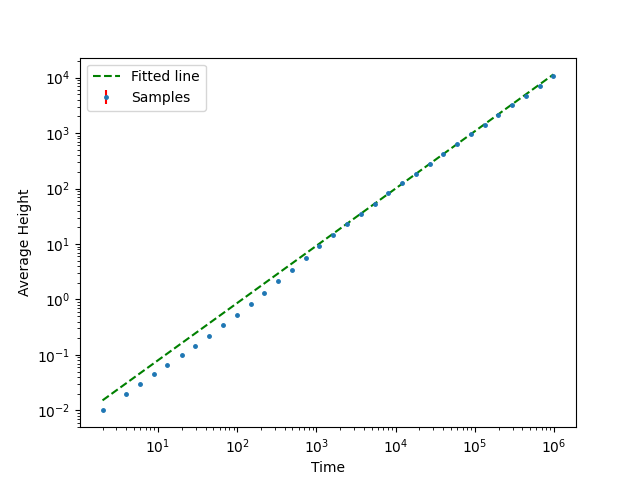
\includegraphics[width=\textwidth]{q6_200_50_1_14_.4_avg.png}
    \caption{منحنی تغییرات میانگین ارتفاع بر حسب زمان برای کنارنشستی به طول $200$ و با $50$ بار تکرار}
    \label{fig:q6_200_50_avg}
  \end{minipage}
\end{figure}

\begin{table}[h]
	\centering
	\begin{tabular}{|c|c|c|c|}
    \hline
    \text{طول } ($l$) & \text{میانگین ارتفاع} & \text{ناهمواری } ($\omega$) & \text{اشباع } ($\omega_s$) \\
    \hline
    $250$ & $1.0261 \pm 10^{-4}$ & $\beta = 0.2346 \pm 10^{-4}$ & $7.94 \pm 10^{-2}$ \\
    \hline
    $200$ & $1.0322 \pm 10^{-4}$ & $\beta = 0.219 \pm 10^{-3}$ & $7.14 \pm 10^{-2}$ \\
    \hline
    $150$ & $1.0398 \pm 10^{-4}$ & $\beta = 0.2113 \pm 10^{-4}$ & $6.436 \pm 10^{-3}$ \\
    \hline
    $100$ & $1.0703 \pm 10^{-4}$ & $\beta = 0.242 \pm 10^{-3}$ & $5.177 \pm 10^{-3}$ \\
    \hline
	\end{tabular}
	\caption{شیب خطوط فیت شده به منحنی تغییرات میانگین ارتفاع و ناهمواری و مقدار اشباع برای طول‌های مختلف کنارنشست}
	\label{tab:q6_slope}
\end{table}

\begin{figure}[h]
  \centering
  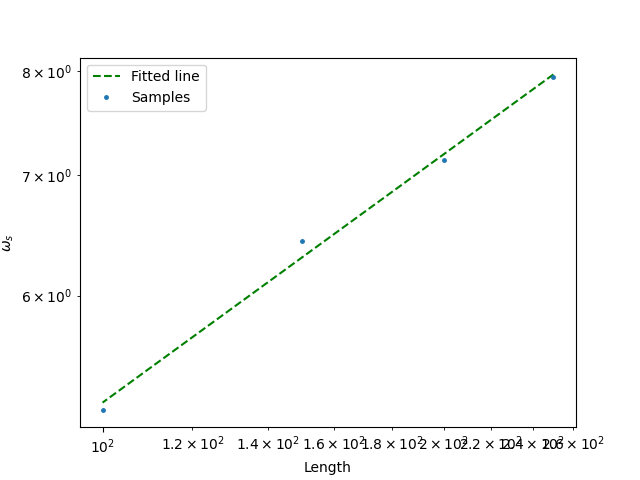
\includegraphics[width=.5\textwidth]{q6_z.png}
  \caption{منحنی تغییرات اشباع بر حسب طول کنارنشست}
  \label{fig:q6_z}
\end{figure}


\section{\textbf{ول‌نشست رقابتی}}
کد این بخش از تمرین در فایل
\lr{q7.py}
قابل مشاهده است. روش کار به این صورت است که ابتدا یک
\lr{object}
از کلاس
\lr{NearestNeighborBallisticDepositionWithInitialCondition}
با طول دلخواه می‌سازیم. سپس تابع
\lr{render}
را با زمان مورد نظر فراخوانی می‌کنیم. روش کار این تابع به این صورت است که روی بازه‌های زمانی داده شده
پیمایش می‌کند و در هر بازه، به اندازه‌ی طول آن، اعداد تصادفی از مجموعه اندیس‌ها تولید می‌کند. 
سپس روی این اندیس‌های تصادفی پیمایش می‌کند و بیش‌ترین ارتفاع را در همسایگی آن، در صورتی که غیر صفر باشد، پیدا کرده و ارتفاع آن خانه را برابر با آن قرار می‌دهد.
در نهایت داده‌های به دست آمده را در یک فایل به فرمت
\lr{.npy}
ذخیره می‌کند.
برای رسم تصویر داده‌ها باید تابع
\lr{show}
را صدا بزنیم.
تصویر به دست آمده برای طول
$200$
و زمان
$18\,000$
را در شکل
\ref{fig:q7_200_18000}
می‌توان مشاهده نمود.
\\
برای ایجاد یک آنسامبل آماری، می توانیم تابع
\lr{make$\_$ensemble}
را با بازه‌ی زمانی و تعداد دلخواه فراخوانی کنیم. 
این تابع به تعداد داده شده، تابع
\lr{render}
را صدا می‌زند و در نهایت میانگین ارتفاع و 
$\omega$
را برای این آنسامبل محاسبه کرده و در یک فایل ذخیره می‌کند.
برای انجام تحلیل بر روی این داده‌های به دست آمده و محاسبه شیب رشد، تابع
\lr{analyse}
را صدا می‌زنیم.
منحنی تغییرات عرض، میانگین ارتفاع و ناهواری بر حسب زمان را برای کنارنشستی رقابتی به طول
$200$
و با
$100$
تکرار را در شکل‌های
\ref{fig:q7_200_100_width}
و
\ref{fig:q7_200_100_avg}
و
\ref{fig:q7_200_100_omega}
می‌توان مشاهده نمود.
\\
شیب خط فیت شده به این سه منحنی را در جدول
\ref{tab:q7_slope}
همراه با خطا‌ی محاسبه‌شان آورده شده است.
همان‌طور که دیده می‌شود، نماهای بحرانی کاملا متفاوتی نسبت به باقی مدل‌های بررسی شده دارد.

\begin{figure}[h]
  \centering
  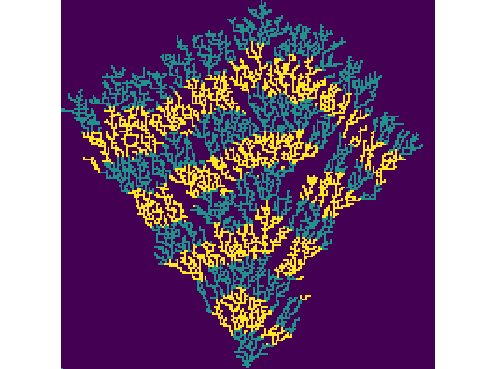
\includegraphics[width=.5\textwidth]{q7_200_18000.png}
  \caption{ول‌نشست رقابتی به طول $200$ و زمان $18\,000$}
  \label{fig:q7_200_18000}
\end{figure}

\begin{figure}[h]
	\centering
  \begin{minipage}[b]{0.48\textwidth}
    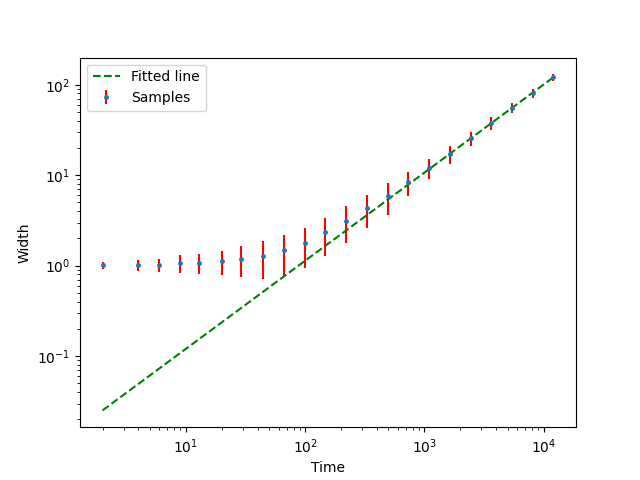
\includegraphics[width=\textwidth]{q7_200_100_1_9.5_.4_width.png}
    \caption{منحنی تغییرات عرض بر حسب زمان برای کنارنشستی رقابتی به طول $200$ و با $100$ بار تکرار}
    \label{fig:q7_200_100_width}
  \end{minipage}
  \hfill
  \begin{minipage}[b]{0.48\textwidth}
    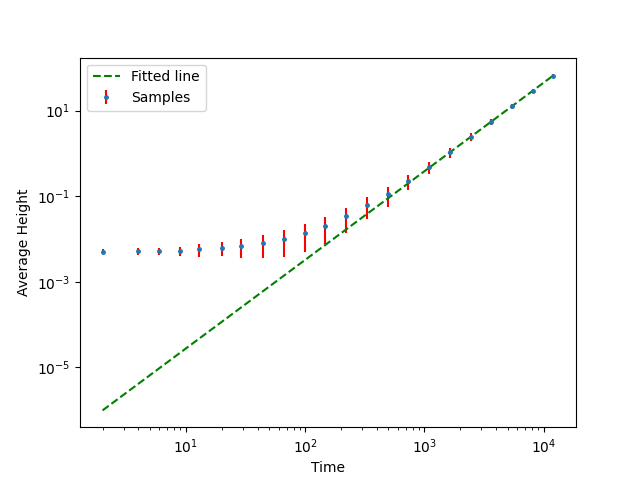
\includegraphics[width=\textwidth]{q7_200_100_1_9.5_.4_avg.png}
    \caption{منحنی تغییرات میانگین ارتفاع بر حسب زمان برای کنارنشستی رقابتی به طول $200$ و با $100$ بار تکرار}
    \label{fig:q7_200_100_avg}
  \end{minipage}
  \hfill
  \begin{minipage}[b]{0.48\textwidth}
    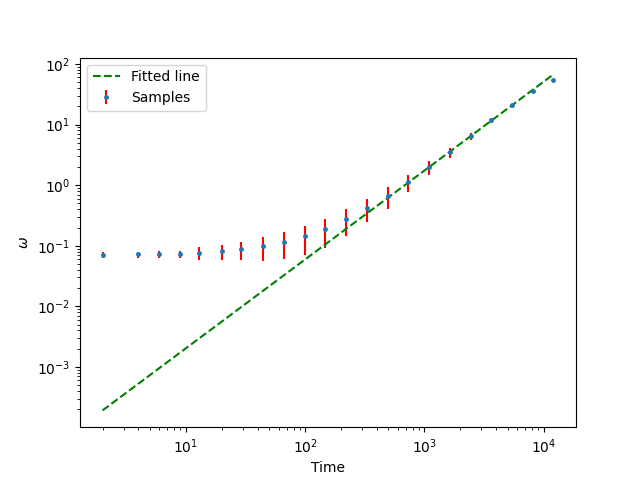
\includegraphics[width=\textwidth]{q7_200_100_1_9.5_.4_omega.png}
    \caption{منحنی تغییرات ناهمواری بر حسب زمان برای کنارنشستی رقابتی به طول $200$ و با $100$ بار تکرار}
    \label{fig:q7_200_100_omega}
  \end{minipage}
\end{figure}

\begin{table}[h]
	\centering
	\begin{tabular}{|c|c|}
		\hline
    $2.0697 \pm 10^{-4}$ & \text{میانگین ارتفاع} \\
     \hline
    $0.97357 \pm 10^{-5}$ & \text{عرض} \\
     \hline
    $\beta = 1.4663 \pm 10^{-4}$ & \text{ناهمواری } ($\omega$) \\
    \hline
	\end{tabular}
	\caption{شیب خطوط فیت شده به منحنی تغییرات میانگین ارتفاع و عرض ول‌نشستی رقابتی به طول ۲۰۰}
	\label{tab:q7_slope}
\end{table}

\end{document}
